%% Template article for Elsevier's document class `elsarticle'
%% with numbered style bibliographic references
\documentclass[preprint,12pt]{elsarticle}

\usepackage{setspace}
\doublespacing

\usepackage{hyperref}


% remove preprent footnote
\makeatletter
\def\ps@pprintTitle{%
 \let\@oddhead\@empty
 \let\@evenhead\@empty
 \def\@oddfoot{\centerline{\thepage}}%
 \let\@evenfoot\@oddfoot}
\makeatother

%% Use the option review to obtain double line spacing
%% \documentclass[preprint,review,12pt]{elsarticle}

%% Use the options 1p,twocolumn; 3p; 3p,twocolumn; 5p; or 5p,twocolumn
%% for a journal layout:
%% \documentclass[final,1p,times]{elsarticle}
%% \documentclass[final,1p,times,twocolumn]{elsarticle}
%% \documentclass[final,3p,times]{elsarticle}
%% \documentclass[final,3p,times,twocolumn]{elsarticle}
%% \documentclass[final,5p,times]{elsarticle}
%% \documentclass[final,5p,times,twocolumn]{elsarticle}

\usepackage{graphicx}
\usepackage{amssymb}
\usepackage{amsmath}
\usepackage{caption}

\biboptions{comma,round}

% shortcuts
\newcommand{\bbeta}{\boldsymbol{\beta}}
\newcommand{\blambda}{\boldsymbol{\lambda}}
\newcommand{\T}{\intercal}
\newcommand{\bS}{\mathbf{S}}
\newcommand{\bQ}{\mathbf{Q}}
\newcommand{\bSigma}{\boldsymbol{\Sigma}}
\newcommand{\bm}{\boldsymbol}  % bold maths symbols
\newcommand{\tl}{\tilde{\lambda}}   % thinned little lambda
\newcommand{\tL}{\tilde{\Lambda}}  % thinned big lambda


\DeclareMathOperator*{\argmax}{arg\,max}  % * means _ puts thing beneath operator

\begin{document}
\begin{frontmatter}
\title{Point transect distance sampling in inlabru}

%% use the tnoteref command within \title for footnotes;
%% use the tnotetext command for the associated footnote;
%% use the fnref command within \author or \address for footnotes;
%% use the fntext command for the associated footnote;
%% use the corref command within \author for corresponding author footnotes;
%% use the cortext command for the associated footnote;
%% use the ead command for the email address,
%% and the form \ead[url] for the home page:
%%
%% \title{Title\tnoteref{label1}}
%% \tnotetext[label1]{}
%% \author{Name\corref{cor1}\fnref{label2}}
%% \ead{email address}
%% \ead[url]{home page}
%% \fntext[label2]{}
%% \cortext[cor1]{}
%% \address{Address\fnref{label3}}
%% \fntext[label3]{}


%% use optional labels to link authors explicitly to addresses:
%% \author[label1,label2]{<author name>}
%% \address[label1]{<address>}
%% \address[label2]{<address>}

\author{Andrew E Seaton}

\address{Centre for Research into Ecological \& Environmental Modelling and School of Mathematics \& Statistics, University of St Andrews, St Andrews, Fife, Scotland}

\begin{abstract}
Point transect distance sampling in \texttt{inlabru}
\end{abstract}

%\begin{keyword}
%Distance sampling \sep Stochastic partial differential equations \sep Integrated nested Laplace approximation \sep Generalized additive model
%\end{keyword}
\end{frontmatter}

\section*{Introduction}

Introduction outline:
\begin{enumerate}
	\item Estimation of abundance and spatial distribution of animals is an important topic
	\item Distance sampling is a family of methods that aim to do this whilst accounting for imperfect detectability of animals
	\item Distance sampling began life under a design-based inference paradigm
	\item Randomised survey design is used in two ways.  Firstly, to justify the assumption that the true distribution of animals is uniform with respect to distance from the observer.  Secondly, to construct Horvit-Thompson-like estimators of animal density, which are then converted to abundance estimates for regions of interest
	\item Interest in the spatial distribution of animals has led to the development of approaches that combine traditional distance sampling methods and spatially explicit generalized additive models
	\item In this approach the estimated detection probabilities for discrete spatial units are used as an offset in a generalized additive model where the response variable is a count of detections within each unit
	\item This two-stage approach needs a way to propogate uncertainty from the detection model to the spatial model
	\item Recently [[JOYCE PAPER]] presented a one-stage approach that simultaneously estimates the detection and spatial processes, avoids binning data into counts and removes the need to consider uncertainty propagation
	\item This approach considered line-transect distance sampling as thinned log-Gaussian Cox process
	\item To estimate the detection function [[JOYCE et al]] constructed a spline-like function using an SPDE approach and fit the model using \texttt{R-INLA}
	\item In this paper we show how to achieve a similar one-stage model for point transect distance sampling
	\item Point transect surveys require a different approach than line transects because the area surveyed increases with distance from observer
	\item In addition to accounting for this we present an alternative way to specify the detection function.  We replace the spline approach with a parametric family of detection functions such as half-normal and hazard rate functions
	\item  These detection functions are typically not linear in their parameters and so cannot be straightforwardly estimated using methods for additive linear predictors
	\item To solve this we implement an iterative approach based on a Taylor approximation of the detection function and fit the model using the \texttt{inlabru} package which extends the functionality of \texttt{R-INLA}
	\item This represents a novel development in distance sampling methods that allows simultaneous estimation of parametric detection functions and the spatial distribution of animals from point transect data
\end{enumerate}

\section*{Distance Sampling as a Thinned Point Process}

We assume the location of animals are a point pattern that follows a log-Gaussian Cox process with intensity process $\lambda(s)$.  The log-Gaussian Cox process is a flexible approach that can include spatially structured random effects on the intensity process to account for unexplained heterogeneity not captured by fixed effect covariates.  

\sloppy For the case with imperfect detection of points we specify a thinning probability function $g(s) = \mathbb{P}(\text{a point at $s$ is detected})$. A key property of the log-Gaussian Cox process is that a realisation thinned with thinning probability function $g(s)$ also follows a log-Gaussian Cox process with intensity given by $\tl(s) = \lambda(s)g(s)$.  

Standard distance sampling approaches specify $g(s)$ as a function that decays with increasing distance from the observer.  For example, if $r(s)$ denotes the distance of a point at $s$ from the observer, the half-normal thinning probability function is $g(s | \sigma) = \exp(-r(s)^2 / 2\sigma^2)$ where $\sigma$ is a variance parameter to be estimated using the observed distances.  The parameter $\sigma$ can only be estimated if some assumption is made about the intensity of the animal locations.  Without such an assumption detectability and intensity are confounded.  The standard assumption of distance sampling is that the intensity is constant with respect to changes in $r(s)$.  Thus any observed differences from uniformity can be attributed to detectability, and not variation in the intensity.  

A point transect distance sampling survey consists of a set of $K$ sampled regions.  The $k$-th sampled region we denote $\Omega_k \subset \mathbb{R}^2$ and the total surveyed region $\Omega = \cup_{k=1}^K \Omega_k$.  For simplicity we assume that all sampled regions are discs with radius $W$ and $\Omega_j \cap \Omega_k = \emptyset$ for all $j \neq k$.  The thinning probability function $g(s)$ is then defined relative to the positions of the surveyed regions.  The probability of observing a point outside the surveyed region is zero.  We denote the probability of observing a point $s \in \Omega_k$ as $g_k(s)$.  Since the surveyed regions are non-overlapping each location $s$ is associated with a single thinning probability function $g_k$.  For example, for an observer at location $s_k \in \Omega_k$, the half-normal thinning probability function is $g_k(s) = \exp(-\lVert s - s_k \rVert_2^2 / 2\sigma^2)$. The assumption of non-overlapping survey regions can be relaxed by including extra information such as the time of each observation.  For simplicity we do not consider this here.  The thinning probability function for any $s \in \Omega$ is then given by $g(s) = g_{k(s)}(s)$ where $k(s) = k$ for $s \in \Omega_k$.  

The likelihood of observed points at locations $\bm{Y} = (s_1, \ldots, s_n)^\intercal$ is then
\begin{equation}
\label{lgcp-likelihood}
\pi(\bm{Y} | \theta, \phi) = \exp\left(-\int\displaylimits_{s \in \Omega} \lambda(s) g(s) \mathrm{d}s \right)\prod_{i=1}^n \lambda(s_i)g(s_i)
\end{equation}

The integral component of the likelihood does not usually have analytical solutions.  Replacing the integral with a weighted sum allows the log-likelihood to be rewritten as a weighted Poisson log-likelihood.  

To evaluate the integral we introduce polar coordinates notation $s_k(r, \theta) = s_k + r\left[\cos\theta, \sin\theta \right]^T$ to represent locations in each sampling unit $\Omega_k$.   In general the thinning function depends only on $r$ and not on $\theta$.  We assume this is the case in the following and use the shorthand $g_k(r) = g(s_k(r, \theta))$. It follows that the integral can be rewritten as a sum of weighted one-dimensional integrals $\sum_{k=1}^K 2\pi \lambda(s_k) \int_0^W r g_k(r)\mathrm{d}r$ using the assumption that $\lambda(s)$ is constant within each sampling unit.  For each sampling unit we approximate the one-dimensional integral using a midpoint integration method with $M$ integration locations $r_{k1}, \ldots, r_{kM}$ and associated weights $\alpha_{k1}, \ldots, \alpha_{kM}$.  This gives
\begin{equation*}
	\int\displaylimits_{s \in \Omega} \lambda(s)g(s)\mathrm{d}s \approx \sum_{k=1}^K \sum_{j=1}^M \tilde{\alpha}_{kj} \tl(s_{kj}) 
\end{equation*}
where $\tilde{\alpha}_{kj} = 2\pi \alpha_{kj}r_{kj}$ and $\tl(s_{kj}) = \lambda(s_k) g_k(r_{kj})$.  

To simplify notation below we let $\tilde{\alpha}_{k} = (\alpha_{k1}, \ldots, \alpha_{kM})^\intercal$ and $\tilde{\alpha} = (\alpha_1^\intercal, \ldots, \alpha_K^\intercal)^\intercal$.  Similarly let $\tl_k = (\tl(s_{k1}), \ldots, \tl(s_{kM}))^\intercal$, $\tl_{int} = (\tl_1^\intercal, \ldots, \tl_K^\intercal)^\intercal$ and denote the intensity evaluated at the observed locations as $\tl_{obs} = (\tl(s_1), \ldots, \tl(s_n))^\intercal$

Then the approximate log-likelihood is

\begin{equation}
\label{approx-log-likelihood}
	\log \pi(\bm{Y}) \approx - \tilde{\alpha}^\intercal \tl_{int} + 1^\intercal\log\tl_{obs}
\end{equation}

This approximation can be written as a modified Poisson likelihood.  To see this let $\exp \eta = (\tl_{int}^\intercal, \tl_{obs}^\intercal)^\intercal$, 
$\alpha = (\tilde{\alpha}^\intercal, 0_{n \times 1}^\intercal)^\intercal$ and construct a vector of pseudo-observations $y = (0_{KM\times 1}^\intercal, 1_{n \times 1}^\intercal)^\intercal$.  Then the approximate likelihood becomes
\begin{equation}
\pi(\bm{Y}) \approx \prod_{i=1}^{KM + n} \eta_i^{y_i}\exp(-\alpha_i\eta_i)
\end{equation}

This is similar to a Poisson likelihood with an offset term equal to $\log\alpha$.


\section*{Intensities for incomplete data}

In the above we assume the data are complete records of animal location.  However, in many distance sampling surveys the exact location of the animal is not recorded - instead only the location of the observer and the distance to the observer are recorded.  Data of this type can be analysed within a point process framework by deriving the appropriate intensity function for the incomplete data.

Using the polar coordinates notation given above, for true animal location $s_k(r, \theta) \in \Omega_k$, we consider the case where we observe $r$ but not $\theta$.  It follows that the intensity for points at a distance $r$ observed within sampling unit $\Omega_k$ is
\begin{align}
\tl_k(r) &= \oint\displaylimits_{c_k(r)} \lambda(s)g_k(s)\mathrm{d}s \nonumber \\
&= 2\pi\lambda(s_k)rg_k(r)
\end{align}
 where $c_k(r)$ is a circle of radius $r$ centred at $s_k$ and the second line follows from changing to polar coordinates and the assumption of constant intensity within $\Omega_k$.  This intensity differs from the full data case by including the $2\pi$  term to account for the fact that we do not observe $\theta$ and the additional $r$ term to account for the increasing area surveyed at larger distances.  
 
\section*{Modelling $\lambda(s)$ using the stochastic partial differential equation approach}

To model the intensity of animal locations we use a combination of fixed effects of spatial covariates and a spatially structured random effect.  This allows us to associate distance sampling data with environmental and ecological conditions that may be relevant to understanding the ecology of the species of interest.  For cases where we have insufficient covariates to fully explain the location of animals the spatially structured random effect accounts for additional heterogeneity in the intensity and is required to assume conditional independence between points, given the intensity.  

The log-intensity of animal locations is given by
\begin{equation*}
\log \lambda(s) = \beta_0 + \sum_v \beta_v z_v(s) + \xi(s)
\end{equation*}
where $\beta_0$ is an intercept parameter, the $z_v(s)$ are spatially indexed covariates with effect parameters $\beta_v$ and $\xi(s)$ is a zero-mean Gaussian random field with Mat\'ern covariance
\begin{equation}
C(s_1,s_2) = \frac{2^{1-\nu}}{4\pi\kappa^2\tau^2\Gamma(\nu)}(\kappa \|s_1-s_2\|)^{\nu}K_\nu(\kappa \|s_1-s_2\|)
\end{equation}
where \(\nu, \kappa, \tau\) are parameters and \(K_{\nu}\) is the modified Bessel function of the second kind.  All three parameters are not simultaneously identifiable and it is conventional to assume a value for $\nu$ which controls the mean-square differentiability of the process.  We set $\nu = 1$ which is the most common default value in the approximation approach outlined below.  [[Would like to justify $\nu = 1$ somehow]]

We use a Gaussian Markov random field approximation of $\xi(s)$ following the approach of [[Lindgren 2011]] based on specifying $\xi(s)$ via a stochastic partial differential equation.  Given a finite element mesh on the spatial domain with $L$ nodes and associated piece-wise linear basis functions $\phi_1, \ldots, \phi_L$ we represent $\xi$ as $\xi(s) = \sum_l \xi_l \phi_l(s)$.  The parameters $\xi_1, \ldots, \xi_L$ follow a multivariate normal distribution with sparse precision matrix $\bm{Q}_{\xi} = \frac{1}{\tau^2}\left(\kappa^4\bm{C} + 2\kappa^2\bm{G_1} + \bm{G_2}\right)$ where $\bm{C}$, $\bm{G_1}$, $\bm{G_2}$ are all sparse matrices the elements of which are defined via an approximate solution to a stochastic partial differential equation. The precision parameter $\tau$ controls the marginal variance of the field and $\kappa$ is an inverse range parameter that controls the rate of decay of the covariance as distance between locations increases.  Further details of this Gaussian Markov random field approximation are given in the supplementary materials. 

\section*{Thinned Intensities} 

The above specifies a model for all animal locations in the area of interest.  The log-intensity for observed points is $\log\tl(s) = \log\lambda(s) + \log g(s)$.  This presents a problem since $\log g(s)$ is not typically linear in its parameters. However, for any single set of parameter values, $g(s)$ is essentially an offset term.  That is to say, if we could specify $g(s)$ as known then we could proceed with inference with a standard additive linear predictor.   

TO DO:

\begin{itemize}
 \item Description of iterated INLA here
\end{itemize}


\section*{Case-Study:  Hawaiian Akepa Survey}

Section outline:
\begin{enumerate}
	\item Introduce the Akepa data, survey method, conservation status, conservation approaches, questions managers have.
	\item Example code snippets for how to specify the model in inlabru
	\item This includes discussion of priors.  Reference PC-priors, short description of how they work and why they are important for spatial modelling with Gaussian random fields.  In this case:  the prior for the range parameter was chosen based on the smallest distance between sampled locations.  The prior for sigma was based on a plausible scale for the maximum intensity.  
	\item Show main results:  (i) The posterior mean of intensity (ii) The CV of the posterior intensity (iii)  The expected abundance
	\item Discussion of difference between \textit{expected} abundance and \textit{realized abundance}.  Show how we create a posterior for realized abundance by monte-carlo sampling and averaging of Poisson probability mass functions.  Highlight that this is not often considered and is a natural thing to do in Bayesian setting where it is possible to draw monte-carlo samples from the posterior.  Plots of posterior for expected and realized abundance.  Note extra variation in realized abundance over expected abundance.  
	\item Plot lower 0.025 quantile and upper 0.975 quantile of intensity.  Note the problem of multiple hypothesis testing and that these maps may be misleading.  Describe the excursion sets approach to solving this problem.
	\item Show plots of estimated excursion sets for various thresholds and emphasise the usefulness from a management point of view.  Emphasise the \textit{joint} probability of every location in the set exceeding a threshold.
	\item A small comparison with the GAM approach (perhaps in an appendix?) to show the similarity for the mean intensity.  Compare the uncertainty.  Reassuring that the methods agree.    
\end{enumerate}

\newpage

TODO HERE:  Description of Akepa data, survey method, key questions, what do we care about from ecology/conservation point of view.  Then, code snippets of how to specify the model in inlabru, brief discussion of PC priors and how they were chosen here

\bigskip

The predicted mean of the posterior intensity is shown in \autoref{fig:intensity-mean-cv} along with a map of the coefficient of variation (CV) of the posterior intensity field on a regular prediction grid with cell area of approximately 1.7 hectares.  This shows a region of high intensity in the south and much lower intensity in the north.  The CV plot shows clearly that there is less variation in the posterior intensity field in areas with greater sampling effort.  In general the south, with greater density of sampled locations, has a lower CV than the north, where sampling units are more spread out.  The areas of highest CV are those regions furthest away from any sampled location, reflecting the intuitive fact that we are least certain in areas where we did not look.   

\begin{figure}
	\includegraphics[scale=0.5]{figures/intensity_mean_cv.png}
	\caption{(left) Posterior mean of the intensity (right) Posterior coefficient of variation of the intensity}
	\label{fig:intensity-mean-cv}
\end{figure}

The CV plot shows a measure of uncertainty relative to the mean intensity in each prediction grid cell.  However, often we are interested in the uncertainty around the mean intensity on the scale of the intensity function itself - perhaps seeking to identify areas where we can confidently predict particularly high or low intensities.  To attempt to communicate this uncertainty around the mean it is common [[references?]] to present the lower and upper quantiles corresponding to a 95\% credible interval for each prediction cell (\autoref{fig:intensity-quantiles}).  

\begin{figure}
	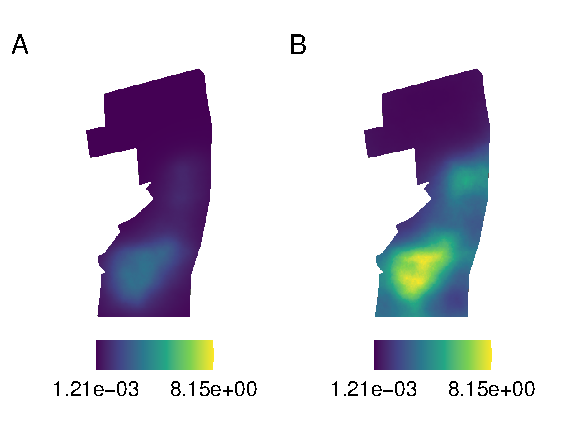
\includegraphics[scale=0.5]{figures/intensity_quantiles.png}
	\caption{The predicted posterior intensity summarised in three plots by the mean (upper),  0.025 quantile (lower left) and 0.975 quantile (lower right) for each prediction grid cell.  All three plots use a common colour scale}
	\label{fig:intensity-quantiles}
\end{figure}

We believe quantile plots like those in \autoref{fig:intensity-quantiles} to be challenging to interpret and potentially misleading.  The temptation is to interpet these plots as showing possible intensity surfaces that produced the observed data.  We believe this misconception would be extremely common in particular for non-statistically trained audiences. The maps in \autoref{fig:intensity-quantiles} in fact only show \textit{summary statistics} of a posterior intensity which is specified (in our model) as a log-Gaussian random field.

This difference becomes clear if one generates realizations of the posterior intensity field.  Three such realizations are in \autoref{fig:intensity-realizations}.  There are some notable differences when compared to the mean and quantile summary maps.  First, each realization has finer-grained spatial structure than the mean of the field.  What this means in practice is that we should expect more spatial structure in our collected data than what we might expect if we only look at the posterior mean of the field.  The mean field plot hides the spatial structure the model has been able to estimate from the data.  In general, the mean of a random field will contain less spatial structure than realisations of the field.    

\begin{figure}
	\includegraphics[scale=0.35]{figures/intensity_realized.png}
	\caption{Three realizations of the posterior intensity field}
	\label{fig:intensity-realizations}
\end{figure}

The quantile plots are more concerning.  As mentioned above, the temptation is to interpret these as possible intensities that produced our observed data.  However, they in fact show the quantiles of the \textit{marginal} probability density for each prediction location.  This essentially treats each prediction cell as independent of the others. Whilst any one prediction location may be well described by such quantiles, to present them side by side in one image obscures the fact that the probability that all (or some subset of) the prediction cells would \textit{simultaneously} achieve that value will be in fact much lower than the quantile value and in many cases would be essentially zero.  To demonstrate this we treated the lower and upper quantile plots as though they were intensities and integrated them to obtain an expected abundance estimate of approximately 2500 for the 0.025 quantile and 12,300 for the 0.975.  A naive (and tempting) interpretation of these numbers is as upper and lower limits of the 95\% credible interval for abundance. However, these abundance estimates are essentially impossible according to the estimated posterior for abundance (see \autoref{fig:realized-abundance-posterior}).  This emphasises that the temptation to treat these maps as showing possible intensity surfaces leads to outcomes (and possible management decisions) that are inconsistent with the very model that generated the maps.  

As an alternative we suggest using excursion sets and excursion functions.  This is a recently approach to representing uncertainty in stochastic processes that specifically considers
joint probability of events across multiple locations.  The positive excursion set with level $u$ for a function $f(s)$ with domain $\Omega$ is $A_u^{+}(f) = \{ s \in \Omega ; f(s) < u \}$.  For a stochastic process $\lambda(s)$ the positive excursion set with level $u$ and probability $1 - \alpha$ is 

\begin{equation*}
E_{u,\alpha}^{+}(\lambda) = \argmax_{D}\{\lvert D \rvert : \mathbb{P}\left[D \subset A_u^{+}(\lambda)\right] \geq 1 - \alpha \}
\end{equation*}
It is important to note that $A_u^{+}(f)$ specifies a set for which a function $f(s)$ exceeds a threshold value $u$ for \textit{every location} in the set.  This means that when considering random quantities such as $\lambda(s)$ the definition of the positive excursion set $E_{u,\alpha}^{+}(\lambda)$ is finding the largest such set for which such a condition holds simultaneously for all locations in a region.  Because $\lambda(s)$ is stochastic we must use something akin to a confidence level by specifying $\alpha$.  

Excursion sets can be estimated using...  [[summarise Bolin paper here]]

\autoref{fig:excursion-set} shows the positive excursion set with a level corresponding to 1 bird per hectare with probability 0.95.  This figure can be interpreted in a natural way.  It is the largest possible region for which the intensity is greater than 1 bird per hectare for every location within the region, with probability 0.95.  

\begin{figure}
	\includegraphics[scale=0.5]{figures/excursion_set.png}
	\caption{The positive excursion set with a level corresponding to 1 bird per hectare and probability 0.95}
	\label{fig:excursion-set}
\end{figure}

To visualise multiple such maps we can use the excursion function $F_u^{+}(s) = \sup \{1 - \alpha ; s \in E_{u,\alpha}^+ \}$, which defines for each location something similar to a p-value.  For each $s$ it is the largest possible probability $1 -\alpha$ for which that location would be in the excursion set defined using probability $1 - \alpha$.  The excursion function with a level corresponding to 1 bird per hectare is shown in \autoref{fig:excursion-function}.

\begin{figure}
	\includegraphics[scale=0.5]{figures/excursion_function.png}
	\caption{The positive excursion function with a level corresponding to 1 bird per hectare}
	\label{fig:excursion-function}
\end{figure}

This figure can also be interpreted naturally, defining probabilities each location to be a member of a set for which the probability of exceeding a threshold simultaneously in all locations.  A key feature of these plots is that they display either discrete sub-regions of the area of interest (for excursion sets) or the probability of membership of such discrete sub-regions (for excursion functions).  We believe the risk of interpreting these maps as intensities is much lower than for the quantile plots.  

Another key aim of performing distance sampling surveys is to estimate the abundance of the population of interest.

\begin{figure}
	\includegraphics[scale=0.6]{figures/realized_abundance_posterior.png}
	\caption{Posterior of realized abundance}
	\label{fig:realized-abundance-posterior}
\end{figure}

\begin{figure}
	\includegraphics[scale=0.6]{figures/realized_abundance_vs_exp.png}
\end{figure}

\begin{figure}
	\includegraphics[scale=0.6]{figures/halfnormal.png}
\end{figure}

\newpage

\section*{Discussion}

\begin{enumerate}
	\item Note the model-based Bayesian hierarchical approach provides a framework for working with distance sampling data.  This allows simultaneous estimation of parameters associated with the detection process and the spatial distribution.  It is in principle extendible... somehow...  
	\item Note that Bayesian distance sampling has been done before but that the INLA approach avoids data augmentation and MCMC.  
	\item Iterated INLA is a powerful and flexible way to include non-linear components to a predictor and has applications beyond this application to distance sampling
	\item More to do in future to test how many parameters can be included in the non-linear component and what types of non-linear components are feasible

\end{enumerate}

\end{document}
